% Diebold-Mariano Test Results — Forest Plot
% Replaces: tab:diebold-mariano-tests in section_5way_ensemble_production.tex
% Forest plot showing MAE differences with confidence intervals

\begin{figure}[htbp]
\centering
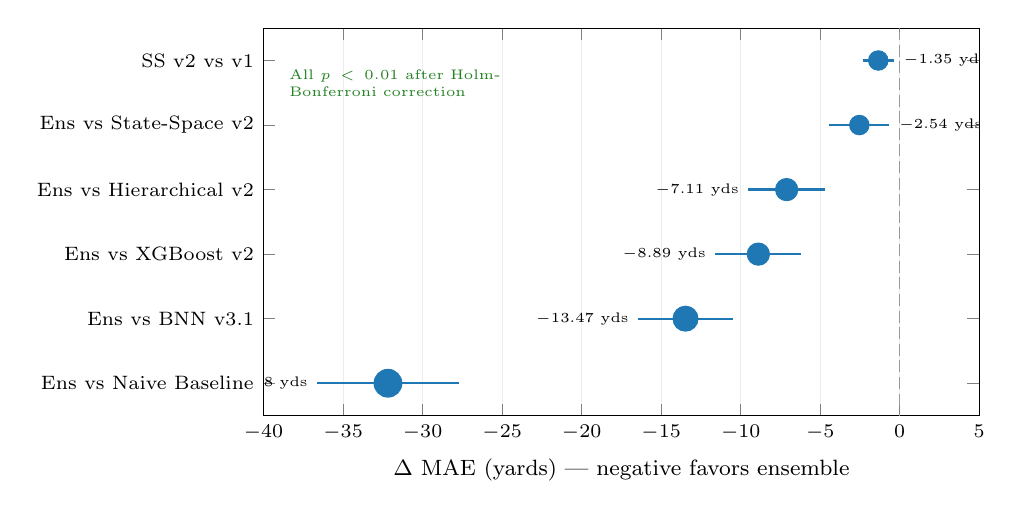
\begin{tikzpicture}
\definecolor{accent}{RGB}{31,119,180}
\definecolor{accentGreen}{RGB}{44,160,44}

\begin{axis}[
  width=0.88\textwidth,
  height=6.5cm,
  xmin=-40, xmax=5,
  xlabel={$\Delta$ MAE (yards) --- negative favors ensemble},
  xlabel style={font=\footnotesize},
  ytick={1,2,3,4,5,6},
  yticklabels={
    {SS v2 vs v1},
    {Ens vs State-Space v2},
    {Ens vs Hierarchical v2},
    {Ens vs XGBoost v2},
    {Ens vs BNN v3.1},
    {Ens vs Naive Baseline}
  },
  yticklabel style={font=\scriptsize},
  y dir=reverse,
  xticklabel style={font=\scriptsize},
  grid=major,
  grid style={gray!15},
  ymajorgrids=false,
  enlarge y limits={abs=0.5},
  extra x ticks={0},
  extra x tick labels={},
  extra x tick style={grid style={black!40, dashed}},
]

% Zero line (no difference)
\draw[black!40, dashed] (axis cs:0,0.3) -- (axis cs:0,6.7);

% CI bars + point estimates
% SS v2 vs v1: -1.35 [-2.33, -0.37]
\draw[accent, thick] (axis cs:-2.33,1) -- (axis cs:-0.37,1);
\addplot[only marks, mark=*, mark size=3.5pt, accent, fill=accent] coordinates {(-1.35, 1)};

% Ens vs SS v2: -2.54 [-4.42, -0.66]
\draw[accent, thick] (axis cs:-4.42,2) -- (axis cs:-0.66,2);
\addplot[only marks, mark=*, mark size=3.5pt, accent, fill=accent] coordinates {(-2.54, 2)};

% Ens vs Hier v2: -7.11 [-9.51, -4.71]
\draw[accent, thick] (axis cs:-9.51,3) -- (axis cs:-4.71,3);
\addplot[only marks, mark=*, mark size=4pt, accent, fill=accent] coordinates {(-7.11, 3)};

% Ens vs XGB v2: -8.89 [-11.59, -6.19]
\draw[accent, thick] (axis cs:-11.59,4) -- (axis cs:-6.19,4);
\addplot[only marks, mark=*, mark size=4pt, accent, fill=accent] coordinates {(-8.89, 4)};

% Ens vs BNN v3.1: -13.47 [-16.44, -10.50]
\draw[accent, thick] (axis cs:-16.44,5) -- (axis cs:-10.50,5);
\addplot[only marks, mark=*, mark size=4.5pt, accent, fill=accent] coordinates {(-13.47, 5)};

% Ens vs Naive: -32.18 [-36.62, -27.74]
\draw[accent, thick] (axis cs:-36.62,6) -- (axis cs:-27.74,6);
\addplot[only marks, mark=*, mark size=5pt, accent, fill=accent] coordinates {(-32.18, 6)};

% Value labels
\node[font=\tiny, anchor=west] at (axis cs:-0.37,1) {$-$1.35 yds};
\node[font=\tiny, anchor=west] at (axis cs:-0.66,2) {$-$2.54 yds};
\node[font=\tiny, anchor=east] at (axis cs:-9.51,3) {$-$7.11 yds};
\node[font=\tiny, anchor=east] at (axis cs:-11.59,4) {$-$8.89 yds};
\node[font=\tiny, anchor=east] at (axis cs:-16.44,5) {$-$13.47 yds};
\node[font=\tiny, anchor=east] at (axis cs:-36.62,6) {$-$32.18 yds};

% All significant annotation
\node[font=\tiny, text=accentGreen!80!black, anchor=north west, align=left, text width=3cm] at (axis cs:-39,1)
  {All $p < 0.01$ after Holm-Bonferroni correction};

\end{axis}
\end{tikzpicture}
\caption[Diebold-Mariano forest plot]{Diebold-Mariano predictive accuracy tests (2022--2024, $n=1{,}405$). Points show MAE differences with 95\% bootstrap CIs. All comparisons significant at $\alpha=0.05$ after Holm-Bonferroni correction. The ensemble outperforms all individual models, with the largest margin against the naive baseline ($-32.18$ yards) and smallest against State-Space v2 ($-2.54$ yards).}
\label{fig:dm-tests-chart}
\end{figure}
